\documentclass{beamer}

\mode<presentation> {

% The Beamer class comes with a number of default slide themes
% which change the colors and layouts of slides. Below this is a list
% of all the themes, uncomment each in turn to see what they look like.

%\usetheme{default}
%\usetheme{AnnArbor}
%\usetheme{Antibes}
%\usetheme{Bergen}
%\usetheme{Berkeley}
%\usetheme{Berlin}
%\usetheme{Boadilla}
%\usetheme{CambridgeUS}
\usetheme{Copenhagen}
%\usetheme{Darmstadt}
%\usetheme{Dresden}
%\usetheme{Frankfurt}
%\usetheme{Goettingen}
%\usetheme{Hannover}
%\usetheme{Ilmenau}
%\usetheme{JuanLesPins}
%\usetheme{Luebeck}
%%\usetheme{Malmoe}
%\usetheme{Marburg}
%\usetheme{Montpellier}
%\usetheme{PaloAlto}
%\usetheme{Pittsburgh}
%\usetheme{Rochester}
%\usetheme{Singapore}
%\usetheme{Szeged}
%\usetheme{Warsaw}

% As well as themes, the Beamer class has a number of color themes
% for any slide theme. Uncomment each of these in turn to see how it
% changes the colors of your current slide theme.

%\usecolortheme{albatross}
%\usecolortheme{beaver}
%\usecolortheme{beetle}
%\usecolortheme{crane}
\usecolortheme{dolphin}
%\usecolortheme{dove}
%\usecolortheme{fly}
%\usecolortheme{lily}
%\usecolortheme{orchid}
%\usecolortheme{rose}
%\usecolortheme{seagull}
%\usecolortheme{seahorse}
%\usecolortheme{whale}
%\usecolortheme{wolverine}

%\setbeamertemplate{footline} % To remove the footer line in all slides uncomment this line
%\setbeamertemplate{footline}[page number] % To replace the footer line in all slides with a simple slide count uncomment this line

\setbeamertemplate{navigation symbols}{} % To remove the navigation symbols from the bottom of all slides uncomment this line
}

\usepackage{graphicx} % Allows including images
\usepackage{booktabs} % Allows the use of \toprule, \midrule and \bottomrule in tables
\usepackage[spanish]{babel}
\usepackage[utf8]{inputenc}
\usepackage{subfig}
\usepackage{color}
\usepackage{soul}
\usepackage{tikz}


%----------------------------------------------------------------------------------------
%	TITLE PAGE
%----------------------------------------------------------------------------------------

\title[Azar e información]{Azar e información} % The short title appears at the bottom of every slide, the full title is only on the title page
\subtitle{¿Qué es el azar?¿Cómo lo medimos?}

\author[C3]{Lucas Puterman} % Your name
\date{\today} % Date, can be changed to a custom date

\begin{document}

\begin{frame}
\titlepage % Print the title page as the first slide
\end{frame}
\begin{frame}
\frametitle{}
\medskip
\begin{figure}[h!]
"Soy de un país vertiginoso donde la lotería es parte principal de la realidad: hasta el día de hoy, he pensado tan poco en ella como en la conducta de los dioses indescifrables o de mi corazón."\\
\textbf{Jorge Luis Borges}, \textit{La lotería en Babilonia}
\end{figure}
\end{frame}

\begin{frame}
\frametitle{Historia del Azar}
\medskip
¿Qué es el azar?\\
\begin{itemize}
	\item La pregunta surge junto con el debate filosófico de determinismo vs. libre albedrío
	\pause
	\item Los griegos se encontraron con la probabilidad, pero no se animaron por miedo a los dioses 
	\pause
	\item Los romanos, fanáticos de los dados, se enfrentaron por primera vez al azar
	\pause
	\item Más adelante se desarrolla el campo de la probabilidad, mientras tanto en la filosofía Leibniz trató el tema
	\pause
	\item El estudio del azar propiamente dicho comienza con Emíle Borel a principios del siglo 20
\end{itemize}
\end{frame}

\begin{frame}
\frametitle{Random?}
\begin{figure}[h!]
\centering
\includegraphics[width=\textwidth,height=\textheight,keepaspectratio]{imagenes/random.png}
\end{figure}
\end{frame}

\begin{frame}
\frametitle{Juego}
\medskip
\begin{figure}[h!]
\centering
\begin{itemize}
	\item Anoten en una hoja un número al azar del 1 al 10
	\pause
	\item Contemos cuantas veces apareció cada uno.
	\pause
	\item ¿Fueron entonces elegidos al azar?
\end{itemize}
\end{figure}
\end{frame}

\begin{frame}
\frametitle{Juego 2}
\medskip

\centering
Pensemos ahora en el azar más simple que conocemos
\pause
\begin{center}
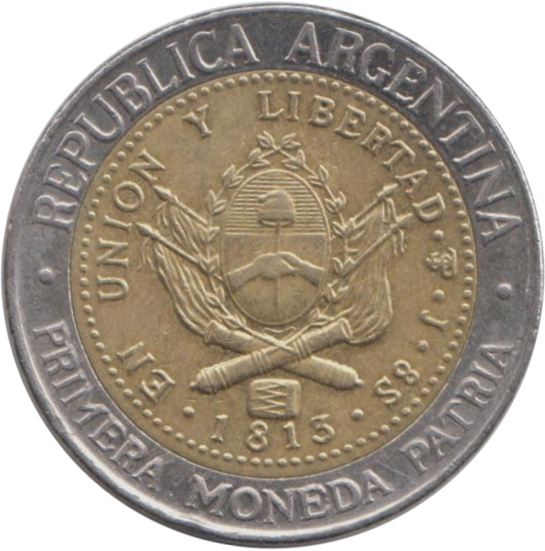
\includegraphics[scale=0.5]{imagenes/peso.jpg}
\end{center}
¿Cómo podemos darnos cuenta si una secuencia infinita de tiradas de monedas es aleatoria?
Hagamos de cuenta que cara = 1 y ceca = 0:
\pause
\begin{itemize}
	\item 111111111111111111111111111111111111111111...
	\pause
	\item 01001000100001000001000000100000001000000001...
	\pause
	\item 100101010110001101110100010010101111001001..
	\pause
	\item ¿Podrían generar una ustedes?
\end{itemize}
Tiene que haber la misma cantidad de caras que de cecas, así como la misma cantidad de combinaciones de tiradas. En caso contrario, podríamos adivinar que va a venir una cantidad infinita de veces!
\end{frame}

\begin{frame}
\frametitle{Definamos Azar}
\medskip
Azar es imposibilidad de adivinar, de predecir, de comprimir...
¿Por quién?\\
\begin{itemize}
	\item Por un humano? \pause \textcolor{red}{No podemos formalizar, dejemoselo a la filosofía}
	\pause
	\item Por una \st{maquina de Turing} computadora \pause \textcolor{blue}{Si! De aquí se formaliza la noción más pura de azar}
	\pause
	\item Por \st{automata finito} algo más simple, sin memoria \pause \textcolor{blue}{Si! Aquí podemos formalizar la noción de normalidad}
\end{itemize}
\end{frame}

\begin{frame}
\frametitle{Normalidad}
\medskip
Borel define tres formas de normalidad en 1909
\begin{itemize}
	\item Un real $x$ es \textcolor{blue}{simplemente normal} en una base si todos sus símbolos aparecen con la misma frecuencia
	\pause
	\item Un real $x$ es \textcolor{blue}{normal} en una base si para cada entero positivo $k$, cada bloque de $k$ digitos aparece con la misma frecuencia
	\pause
	\item Un real $x$ es \textcolor{blue}{absolutamente normal} si es normal en todas las bases.
\end{itemize}
\pause
\begin{tikzpicture}[remember picture,overlay]
\node at (current page.center) {
\includegraphics[width=5cm]{imagenes/signo.png}};
\end{tikzpicture}
\end{frame}

\begin{frame}
\frametitle{Ejemplos}
\medskip
\begin{itemize}
	\item 0.01 002 0003 00004 000005 0000006 00000007 000000008 ... \textcolor{red}{No es simplemente normal en base 10}
	\pause
	\item 0.0123456789 0123456789 0123456789 0123456789 0123456789... \textcolor{red}{Es en base 10, pero no en base 100}
	\pause
	\item Ningún número racional es normal en ninguna base
\end{itemize}
\end{frame}

\begin{frame}
\frametitle{¿$\pi$ es normal?}
\begin{center}
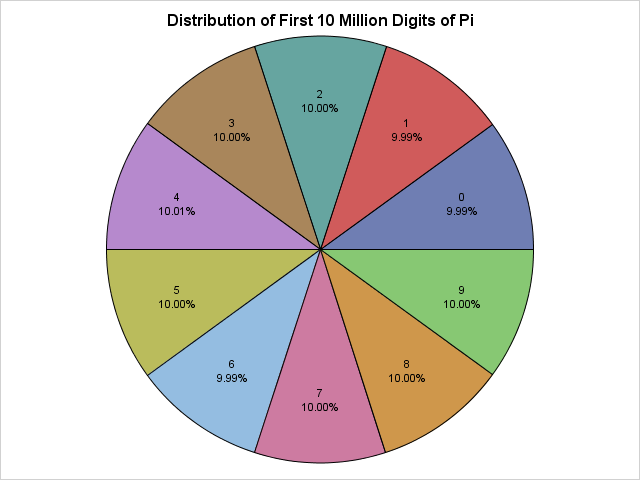
\includegraphics[scale=0.6]{imagenes/digitsofpi.png}
\end{center}
\pause
\begin{tikzpicture}[remember picture,overlay]
\node at (current page.center) {
\includegraphics[width=5cm]{imagenes/signo.png}};
\end{tikzpicture}
\end{frame}

\begin{frame}
\frametitle{$\pi$ es normal?}
Y si $\pi$ fuera normal? Que implicancias tiene?\\
\pause
¿Podrán encontrar su dni adentro de $\pi$?\\
¿Podrán encontrar Hamlet andentro de $\pi$?\\
¿Podrán encontrar Hamlet pero donde el protagonista es Peluffo andentro de $\pi$?\\
\pause
\begin{center}
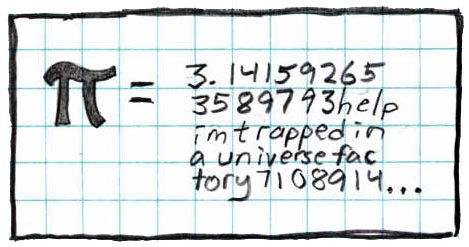
\includegraphics[scale=0.75]{imagenes/piequals.jpg}
\end{center}
\end{frame}

\begin{frame}
\frametitle{La biblioteca de babel, es normal?}
"El universo (que otros llaman la Biblioteca) se compone de un número indefinido, y tal vez infinito, de galerías hexagonales, con vastos pozos de ventilación en el medio, cercados por barandas bajísimas. Desde cualquier hexágono se ven los pisos inferiores y superiores: interminablemente[...]A cada uno de los muros de cada hexágono corresponden cinco anaqueles; cada anaquel encierra treinta y dos libros de formato uniforme;cada libro es de cuatrocientas diez páginas; cada página, de cuarenta renglones; cada renglón, de unas ochenta letras de color negro."
\end{frame}

\begin{frame}
\frametitle{La biblioteca de babel, es normal?}
"Todos los libros, por diversos que sean, constan de elementos iguales: el espacio, el punto, la coma, las veintidós letras del alfabeto. También alegó un hecho que todos los viajeros han confirmado: No hay en la vasta Biblioteca, dos libros idénticos. De esas premisas incontrovertibles dedujo que la Biblioteca es total y que sus anaqueles registran todas las posibles combinaciones de los veintitantos símbolos ortográficos (número, aunque vastísimo, no infinito) o sea todo lo que es dable expresar: en todos los idiomas. Todo: la historia minuciosa del porvenir, las autobiografías de los arcángeles, el catálogo fiel de la Biblioteca, miles y miles de catálogos falsos, la demostración de la falacia de esos catálogos, la demotración de la falacia del catálogo verdadero."\\ \textbf{Jorge Luis Borges}, \textit{La biblioteca de Babel}
\end{frame}

\begin{frame}
\frametitle{La biblioteca de babel, es normal?}
"Todos los libros, por diversos que sean, constan de elementos iguales: el espacio, el punto, la coma, las veintidós letras del alfabeto. También alegó un hecho que todos los viajeros han confirmado: \textcolor{red}{No hay en la vasta Biblioteca, dos libros idénticos.} De esas premisas incontrovertibles dedujo que la Biblioteca es total y que sus anaqueles registran todas las posibles combinaciones de los veintitantos símbolos ortográficos \textcolor{red}{(número, aunque vastísimo, no infinito)} o sea todo lo que es dable expresar: en todos los idiomas. Todo: la historia minuciosa del porvenir, las autobiografías de los arcángeles, el catálogo fiel de la Biblioteca, miles y miles de catálogos falsos, la demostración de la falacia de esos catálogos, la demotración de la falacia del catálogo verdadero."\\ \textbf{Jorge Luis Borges}, \textit{La biblioteca de Babel}
\end{frame}



%\begin{frame}
%\frametitle{Blocks of Highlighted Text}
%\begin{block}{Block 1}
%Lorem ipsum dolor sit amet, consectetur adipiscing elit. Integer lectus nisl, ultricies in feugiat rutrum, porttitor sit amet augue. Aliquam ut tortor mauris. Sed volutpat ante purus, quis accumsan dolor.
%\end{block}
%
%\begin{block}{Block 2}
%Pellentesque sed tellus purus. Class aptent taciti sociosqu ad litora torquent per conubia nostra, per inceptos himenaeos. Vestibulum quis magna at risus dictum tempor eu vitae velit.
%\end{block}
%
%\begin{block}{Block 3}
%Suspendisse tincidunt sagittis gravida. Curabitur condimentum, enim sed venenatis rutrum, ipsum neque consectetur orci, sed blandit justo nisi ac lacus.
%\end{block}
%\end{frame}
%
%%------------------------------------------------
%
%\begin{frame}
%\frametitle{Multiple Columns}
%\begin{columns}[c] % The "c" option specifies centered vertical alignment while the "t" option is used for top vertical alignment
%
%\column{.45\textwidth} % Left column and width
%\textbf{Heading}
%\begin{enumerate}
%\item Statement
%\item Explanation
%\item Example
%\end{enumerate}
%
%\column{.5\textwidth} % Right column and width
%Lorem ipsum dolor sit amet, consectetur adipiscing elit. Integer lectus nisl, ultricies in feugiat rutrum, porttitor sit amet augue. Aliquam ut tortor mauris. Sed volutpat ante purus, quis accumsan dolor.
%
%\end{columns}
%\end{frame}
%
%\begin{frame}
%\frametitle{Table}
%\begin{table}
%\begin{tabular}{l l l}
%\toprule
%\textbf{Treatments} & \textbf{Response 1} & \textbf{Response 2}\\
%\midrule
%Treatment 1 & 0.0003262 & 0.562 \\
%Treatment 2 & 0.0015681 & 0.910 \\
%Treatment 3 & 0.0009271 & 0.296 \\
%\bottomrule
%\end{tabular}
%\caption{Table caption}
%\end{table}
%\end{frame}
%
%%------------------------------------------------
%
%\begin{frame}
%\frametitle{Theorem}
%\begin{theorem}[Mass--energy equivalence]
%$E = mc^2$
%\end{theorem}
%\end{frame}
%
%%------------------------------------------------
%
%\begin{frame}[fragile] % Need to use the fragile option when verbatim is used in the slide
%\frametitle{Verbatim}
%\begin{example}[Theorem Slide Code]
%\begin{verbatim}
%\begin{frame}
%\frametitle{Theorem}
%\begin{theorem}[Mass--energy equivalence]
%$E = mc^2$
%\end{theorem}
%\end{frame}\end{verbatim}
%\end{example}
%\end{frame}
%
%%------------------------------------------------
%
%\begin{frame}
%\frametitle{Figure}
%Uncomment the code on this slide to include your own image from the same directory as the template .TeX file.
%%\begin{figure}
%%\includegraphics[width=0.8\linewidth]{test}
%%\end{figure}
%\end{frame}
%
%%------------------------------------------------
%
%\begin{frame}[fragile] % Need to use the fragile option when verbatim is used in the slide
%\frametitle{Citation}
%An example of the \verb|\cite| command to cite within the presentation:\\~
%
%This statement requires citation \cite{p1}.
%\end{frame}
%
%%------------------------------------------------
%
%\begin{frame}
%\frametitle{References}
%\footnotesize{
%\begin{thebibliography}{99} % Beamer does not support BibTeX so references must be inserted manually as below
%\bibitem[Smith, 2012]{p1} John Smith (2012)
%\newblock Title of the publication
%\newblock \emph{Journal Name} 12(3), 45 -- 678.
%\end{thebibliography}
%}
%\end{frame}
%
%%------------------------------------------------
%
%\begin{frame}
%\Huge{\centerline{The End}}
%\end{frame}

%----------------------------------------------------------------------------------------

\end{document}